\begin{figure}[H]
	\centering
	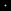
\includegraphics[height = 2in]{../fig/antiyes}
	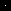
\includegraphics[height = 2in]{../fig/antino}
	
	\caption{A sphere placed so it is encompassed by the viewing volume of only the central pixel is rendered with the default "distributed jitter" antialiasing (left) and with no antialiasing (right).  In this instance, the image with no antialiasing is more photogrammetrically accurate.}
	\label{fig:aliasing}
\end{figure}